% ------------------------------------------------------------
% Page 104
% ------------------------------------------------------------

\underline{Jeannette}, c’est la perle de la classe : curieuse, appliquée, douée sans aucun doute, elle
« avance » très vite J’ai le temps de m’occuper d’elle et à la fin de l’année elle atteint le niveau
d’un bon CM2. Elle sort peu en récréation, préfère lire en classe ou papoter avec mon épouse.
Elle poursuivra ses études à Millau dans de bonnes conditions. Quel a été son avenir ?

\begin{minipage}{\textwidth}
\begin{wrapfigure}{l}{0.27\textwidth}
    \centering
    % Image originale à insérer ici
    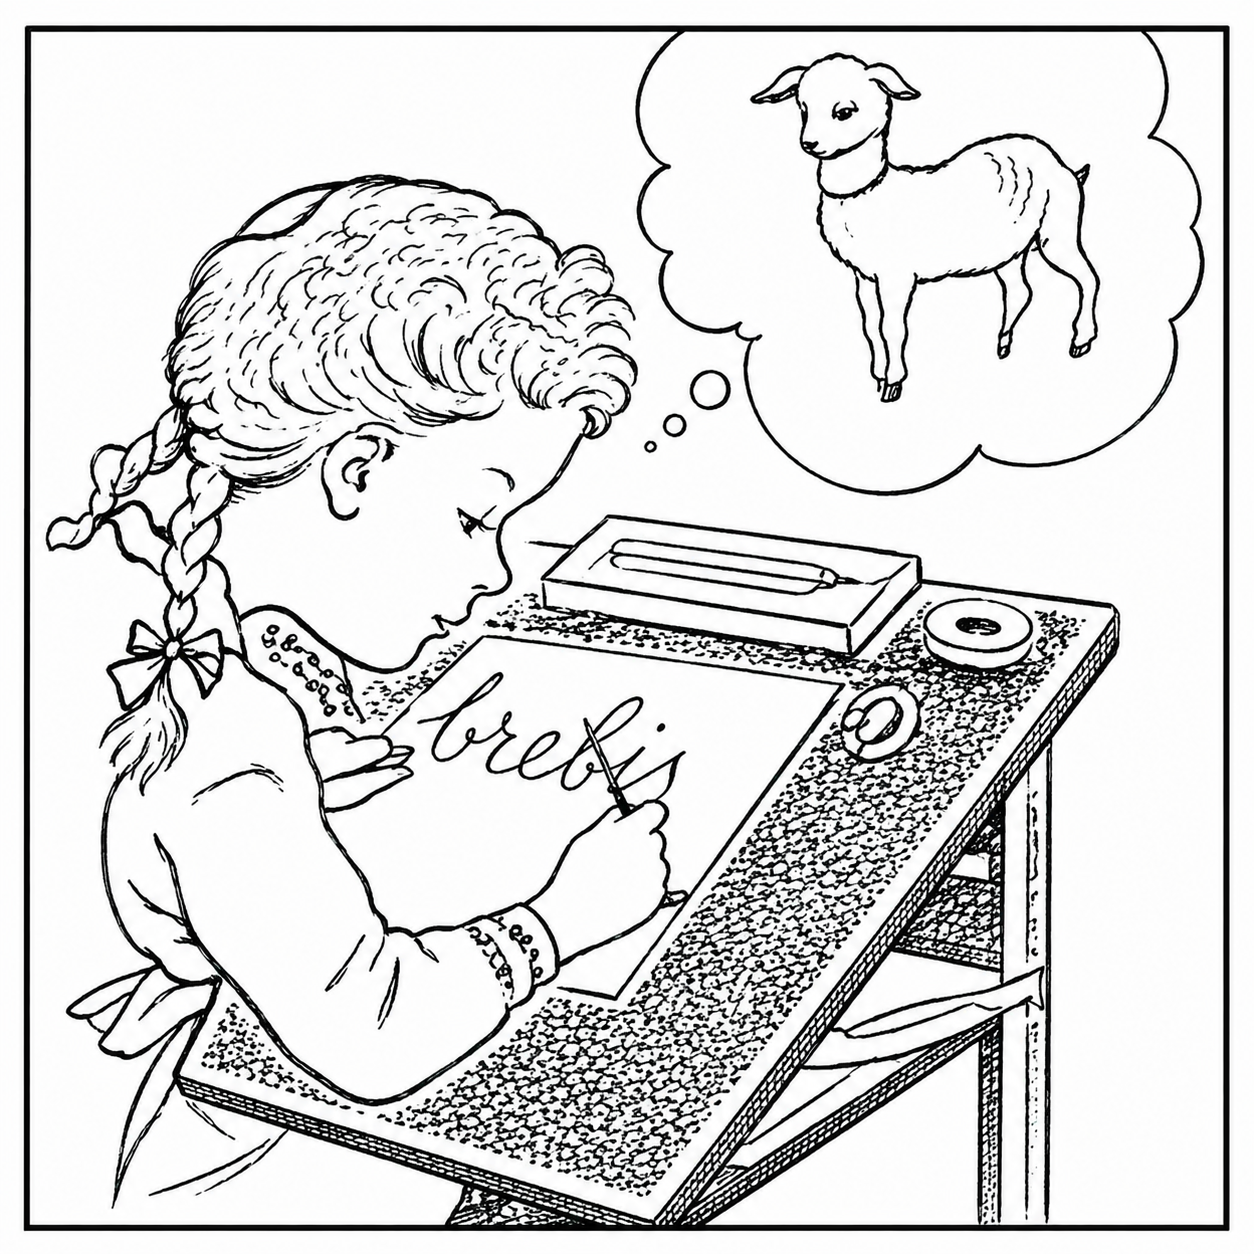
\includegraphics[width=\linewidth]{imgs/111}
\end{wrapfigure}

\textbf{Armandou}, je partage souvent son banc et il est heureux près de
moi. Je travaille à traduire et à franciser son patois. Tout
doucement nous passons des voyelles ... ; aux syllabes et enfin
aux mots qui, parfois, le font rire aux nez dessinons souvent.
J’ai oublié l’infaillible méthode globale de l’Ecole Normale. Mais
Armandou est très appliqué et n’a pas de difficulté en calcul.
Toujours est-il qu’en fin d’année il sait écrire et à peu près lire et
compter. Neuf mois, ce fut long, mais je crois profitable. Qu’est
devenu Armandou ? Il quitta, peu après, le hameau avec sa
famille.
\end{minipage}

\textbf{Le Temple - Ecole. Un peu d’histoire}

Aux lecteurs étonnés de la situation de ce temple-école à Meyrueis (Les Oubrets) je
crois devoir faire part, à posteriori, de mes réflexions, de mes hypothèses aussi, sur
cet état de fait :

Un constat d’abord : sur la rive gauche de la Jonte de nombreux ruisseaux, la Brèze
(le plus important) : le Bétuzon, le Jontanels et bien d’autres rus, s’enfoncent
profondément dans le massif de l’Aigoual. Les petits hameaux, plus ou moins
importants, étaient et sont encore pour ce qu’il en reste, acquis à la Réforme. Ne peut-
on supposer alors, que, très difficiles d’accès, ils ne soient devenus des refuges pour
échapper à la Contre-Réforme du début du 18\ieme{} siècle, à laquelle fut soumise
Meyrueis et la rive droite de la Jonte vers le Causse Méjean ?

Ce petit temple apparaît alors comme une œuvre collective des Huguenots dans le
hameau le plus important « Les Oubrets », facilement accessible aux fidèles par les
sentiers de montagne et apparaît, peut-être, l’idée adjointe de l’utiliser aussi
comme maison d’école pour les enfants d’une communauté protestante
traditionnellement laïque.

D’où une situation confuse et mal définie : temple propriété privée, mais aussi école
publique à fonds publics qui a perduré jusqu’en 1941.
J’ai appris par les habitants du village qu’au moins trois de mes prédécesseurs aux
Oubrets étaient d’origine réformée : Melle B de Rousse, Melle Carrière de Ste Croix-
Vallée- Française et une institutrice de Massevaques dont j’ai oublié le nom.

Et alors... moi-même le seul élève-maître d’origine protestante, d’une promotion de
dix sortants, ne fus-je pas considéré comme le plus à même de s’accommoder de cette
situation particulière ? je me suis souvent posé la question, à laquelle j’éviterai de
répondre : simple hypothèse qui n’engage que moi-même.
